\documentclass[editMode]{ufdissertation}\sloppy
\usepackage[colorlinks=true]{hyperref}
%%%%%%%%%%%%%%%%%%%%%%%%%%%%%%%%%%%%%%%%%%%%%%%%%%%%%%%%%%%%%%%%%%%%%%%%%%%%%%%%
%%%                 User Package and Style File loading.
%%%%%%%%%%%%%%%%%%%%%%%%%%%%%%%%%%%%%%%%%%%%%%%%%%%%%%%%%%%%%%%%%%%%%%%%%%%%%%%%

%\usepackage{CustomMacros}%  This is a user macro/style file.

\usepackage{tikz}%       tikz is used by almost everyone, but certainly by me for this.
\usepackage{pgfplots}%   pgfplots is tikz but better.
%\usepackage{amsrefs}%   amsrefs contains the .bibtex style content for mathematician papers.
\usepackage{algpseudocode}

\usepackage{scrextend}
\deffootnote{1.5em}{0em}{\thefootnotemark\quad}
\usepackage[all]{nowidow} %avoids single lines of text at the top or bottom of page.  If any of your packages cause this package not to work, you will have to manually remove any orphans/widows or add a line penalty
%%%%%%%%%%%%%%%%%%%%%%%%%%%%%%%%%%%%%%%%%%%%%%%%%%%%%%%%%%%%%%%%%%%
%%%                     User Configuration commands
%%%%%%%%%%%%%%%%%%%%%%%%%%%%%%%%%%%%%%%%%%%%%%%%%%%%%%%%%%%%%%%%%%%%%%%%%%%%%%%%

%% Uncomment the relevant line below if you have tables or figures.
\haveTablestrue%        Uncomment this if you have tables in your thesis.
\haveFigurestrue%       Uncomment this if you have figures in your thesis.
\haveObjectstrue%       Uncomment this if you have Objects in your thesis. This is almost certainly not the case however.

%%%%%%%%%%%%%%%%%%%%%%%%%%%%%%%%%%%%%%%%%%%%%%%%%%%%%%%%%%%%%%%%%%%%%%%%%%%%%%%%
%%% Below are the commands to set the degree type, department, graduation time, and chair. 
%       Most of these are self explanatory. 
%       Note: The \chair command takes an optional argument for a cochair. 
%           So if John was your chair and Jacob was a cochair, you would use \chair[Jacob]{John}.
%           If John was your chair and you had no cochair, you can simply use \chair{John}.
%%%%%%%%%%%%%%%%%%%%%%%%%%%%%%%%%%%%%%%%%%%%%%%%%%%%%%%%%%%%%%%%%%%%%%%%%%%%%%%%

\title{Dissertation and Thesis Example File}%  Put your title here.

\degreeType{Doctor of Philosophy}%   Official name of your degree; eg "Doctor of Philosophy".
\major{Mathematics}%                    Your official Department
\author{Jason Nowell}%                  Your Name
\thesisType{Dissertation}%              Dissertation (PhD) or Thesis (Masters)
\degreeYear{2025}%                      Intended graduation year (not the year you submit the thesis)
\degreeMonth{May}%                   Month of graduation should be May, August, or December.
\chair[Jack Griffin]{Claude Rains}%                   Chair and Cochair (see comment block above).

%%%%%%%%%%%%%%%%%%%%%%%%%%%%%%%%%%%%%%%%%%%%%%%%%%%%%%%%%%%%%%%%%%%%%%%%%%%%%%%%
%%% For each of the following, type in the name of the file that contains each section. 
% They are assumed to be tex files, but if they aren't the command takes an optional argument for the extension.
%So, you could load dedication.tex as your dedication file using \setDedicationFile{dedication}
% You could load dedication.txt instead with \setDedicationFile[txt]{dedication}.

% NOTE: For some compilers they may or may not add a .tex to the end of the file automatically.
% If you get a "couldn't find dedication.tex.tex" type error, try the command with an empty optional argument,
%e.g. \setDedicationFile[]{dedication}
%%%
%%%%%%%%%%%%%%%%%%%%%%%%%%%%%%%%%%%%%%%%%%%%%%%%%%%%%%%%%%%%%%%%%%%%%%%%%%%%%%%%

%%% These are REQUIRED sections; easiest to do via these commands.

\setDedicationFile{dedicationFile}%                 Dedication Page
\setAcknowledgementsFile{acknowledgementsFile}%     Acknowledgements Page
\setAbstractFile{abstractFile}%                     Abstract Page (This should only include the abstract itself)
\setReferenceFile{referenceFile}{agsm}%         References. First argument is your bibtex source file
%                                                       the second argument is your bibtex style file.

\setBiographicalFile{biographyFile}%                Biography file of the Author (you).

%%% These are NOT required, so only use them if you actually need/have them.

\setAbbreviationsFile{abbreviations}%           Abbreviations Page
\setAppendixFile{appendix}%                     Appendix Content; hyperlinking might be weird.
\multipleAppendixtrue%                          Uncomment this if you have more than one appendix, 
%                                                   comment it if you have only one appendix.


%%%%%%%                     End of File Assignment
%%%%%%%%%%%%%%%%%%%%%%%%%%%%%%%%%%%%%%%%%%%%%%%%%%%%%%%%%%%%%%%%%%%%%%%%%%%%%%%%

\begin{document}

%%%% Here you just need to include/input your actual work. 
%       The above files (dedication, acknowledgement, titlepage, etc etc) will all be added for you 
%       using the files you assigned above. 
%       If you want to input the above files manually you can comment out the \setFILE command above 
%       and use \input or \include here. Generally you want to use \include to get your pagebreak.
%       NOTE: If you input manually you will have to do some/all the formatting manually.

\renewcommand{\thefootnote}{\fnsymbol{footnote}} % Use symbols for footnotes

\chapter{INTRODUCTION and opening remarks} \renewcommand{\thefootnote}{\fnsymbol{footnote}} % You want an nummbered footnote to mark previously published chapters.
\footnotetext[0]{An un-numbered footnote - this is how you tell the readers that this chapter was previously published and then cite the Journal where it was published. It is typically formatted like "Reprinted with permission from [citation]"\\}\label{intro}


\counterwithin{algorithm}{chapter}
\renewcommand*{\thealgorithm}{\thechapter-\arabic{algorithm}} %Lines 2 and 3 are specifically for those that are using multiple aglorithms in multiple chapters. These must be added to all chapters with algorithms to make the numbering of the objects work correctly. You are welcome to remove if this does not apply to you.

We automatically capitalize all chapters, but if you need to suppress this you can use the class option ``overrideTitles" and/or ``overrideChapter" to allow you to use non-capitalized letters in the title and/or chapter names respectively. For more detailed information on the template's features and options, see the included file ``ufdissertation-Doc-and-Troubleshooting".

 We don't recommend that you change much of anything in the class file unless you're absolutely sure of what your are doing.\renewcommand*{\thefootnote}{\arabic{footnote}}\setcounter{footnote}{0}\footnote{and now we're back to normal footnote marking} 

\section{First-Level Heading or Section Heading}

This is a first-level or Section heading. They should always be in Title-Case. Title case is where all principal words are capitalized except prepositions, articles, and conjunctions. All non-chapter headers must be capitalized manually.

\subsection{Second-Level or Subsection Heading}

This is a second-level or subsection heading. They will always be in title-case but are left-aligned. 

\subsubsection{Third-level or subsubsections}
The third level subheadings are left-aligned but in Sentence case. Only the first letter and any proper nouns are capitalized. 

\subsubsection{If you divide a section, you must divide it into two, or more, parts}
What this means is that if you are going to break down text via subheading, you will want to make sure it is paired with at least one other subheading of the same "level." 

{\bf Paragraph headings.} There is no official fourth level heading. Do not use the Paragraph heading feature in LaTeX, simply apply the bold characteristic to the first few words of a paragraph followed by a colon or period.

\subsection{Subsection}

\(\Omega\) Aliquam mi nisi, tristique at rhoncus quis, consectetur non mi. Phasellus blandit quam ligula, a viverra lacus commodo at. In iaculis nisl vel pretium sollicitudin. In efficitur massa vel elit sollicitudin, vel auctor sapien cursus. Proin feugiat sapien a mi tempus;

\begin{equation}
       X-X'=D+D' 
\end{equation}
Augue sapien mattis leo, nec accumsan turpis quam at neque. Ut pellentesque velit sed
placerat cursus. Integer congue urna non massa dictum, a pellentesque arcu accumsan. Nulla
posuere, elit accumsan eleifend elementum, ipsum massa tristique metus, in ornare neque nisl sed
odio. Nullam eget elementum nisi. Duis a consectetur erat, sit amet malesuada sapien. Aliquam
nec sapien et leo sagittis porttitor at ut lacus. Vivamus vulputate elit vitae libero condimentum
dictum. Nulla facilisi. Quisque non nibh et massa ullamcorper iaculis.
Augue sapien mattis leo, nec accumsan turpis quam at neque. Ut pellentesque velit sed
placerat cursus. Integer congue urna non massa dictum, a pellentesque arcu accumsan. Nulla
posuere, elit accumsan eleifend elementum, ipsum massa tristique metus, in ornare neque nisl sed
odio. Nullam eget elementum nisi. Duis a consectetur erat, sit amet malesuada sapien. Aliquam
nec sapien et leo sagittis porttitor at ut lacus. Vivamus vulputate elit vitae libero condimentum
dictum. Nulla facilisi. Quisque non nibh et massa ullamcorper iaculis.


\begin{quote}
    \begin{singlespace}
  This is an example of a block quote. Aliquam mi nisi, tristique at rhoncus quis, consectetur non mi. Phasellus blandit quam ligula, a viverra lacus commodo at. 
    \end{singlespace}
    
\end{quote}

\subsection{Subsection}

Aliquam mi nisi, tristique at rhoncus quis, consectetur non mi. Phasellus blandit quam ligula, a viverra lacus commodo at. In iaculis nisl vel pretium sollicitudin. In efficitur massa vel elit sollicitudin, vel auctor sapien cursus. Proin feugiat sapien a mi tempus;

\begin{equation}
    X-X'=D+D'
\end{equation}
 
 
\noindent in consequat augue cursus. Nulla sed sagittis purus. Nunc eu consequat orci, eu laoreet enim. Ut euismod tincidunt sem, eget lacinia dui luctus eu. Aliquam mi augue, faucibus id semper vitae, porta ac ligula. Morbi sed ultrices odio. Mauris id luctus ex. Nulla ac libero dictum, interdum turpis lacinia, scelerisque leo. Praesent varius orci ac eros varius pharetra.


\subsection{Subsection}
Donec convallis scelerisque ante, in sollicitudin orci laoreet eu. Nam arcu magna, semper vel lorem eu, venenatis ultrices est. Nam aliquet ut erat ac scelerisque. Maecenas ut molestie mi. Phasellus ipsum magna, sollicitudin eu ipsum quis, imperdiet cursus turpis. Etiam pretium enim a fermentum accumsan. Morbi vel vehicula enim.

\section{Objects}

\begin{algorithm}
\caption[An algorithm with caption]{An algorithm with caption. Example from Overleaf. Change style of Algorithm on line 67 of the .cls file}\label{alg:cap}
\begin{algorithmic}
\Require $n \geq 0$
\Ensure $y = x^n$
\State $y \gets 1$
\State $X \gets x$
\State $N \gets n$
\While{$N \neq 0$}
\If{$N$ is even}
    \State $X \gets X \times X$
    \State $N \gets \frac{N}{2}$  
    \State $y \gets y \times X$
    \State $N \gets N - 1$
\EndIf
\EndWhile
\end{algorithmic}
\end{algorithm}

Please note, the 'Objects' section of this document is based off of the Algorithm environment. If you wish to use external links to a repository, UF recommends using Zenodo (https://guides.uflib.ufl.edu/etds/supplemental). Please reach out to our office at TandDSupport-hd@ufl.edu if you have any questions about adding it to your document, and the ETD team at the library if you have any questions about external repositories (IRManager@uflib.ufl.edu).% Modified from old template.
\chapter{EXAMPLE TABLE FORMATTING} \label{lit}

\section{Table Examples}

 The UF Graduate Counsel is very specific in the Table Requirements.There should be no vertical lines in tables and only three horizontal lines. Tables should be left aligned or the full width of the margins. No bold text, etc., see the web site for the complete list of requirements. One simple improvement can be incorporated by using tabularx instead of the tabular environment. This allows a table to be stretched the full text width easily, which avoids the centered or left aligned issue. Table \ref{sttab} is an example of the tabularx code. 
 
\begin{table}[htbp]% Fix the table captions to sit directly on the table, but figures do NOT sit directly on the figure.
    \captionof{table}[A sample Table using tabularx.]{A sample Table using tabularx. All tables should be left aligned OR the full width of the margin, like this one. }\label{sample}
    \begin{tabularx}{6.5in}{XXX}
      \hline
      First & Second & Third \\
      \hline
      12 & 45 & 26 \\
      17 & 32 & 93 \\
      text & 51 & can be there too. \\	
      \hline
    \end{tabularx}
\end{table}
 
 Praesent fermentum felis nec massa interdum, vel dapibus mi luctus. Cras id fringilla mauris. Ut molestie eros mi, ut hendrerit nulla tempor et. Pellentesque tortor quam, mattis a scelerisque nec, euismod et odio. Mauris rhoncus metus sit amet risus mattis, eu mattis sem interdum.

 \begin{itemize}
      \item First item.
\item Second item.
\item Third item. This item is really long, longer than one line. When the line wraps around in the compiled version, the line
spacing does not match the line spacing throughout the rest of the document.
 \end{itemize}

 \begin{table}[t!]
    \caption{A sample Table using standard tablular}\label{tab}
    \begin{tabular}{c c c}
      \hline
      First & Second & Third \\
      \hline
      12 & 45 & 26 \\
      17 & 32 & 93 \\
      text & 51 & can be there too. \\	
      \hline
    \end{tabular}
\end{table}

\section{Additional Table Examples}
Augue sapien mattis leo, nec accumsan turpis quam at neque. Ut pellentesque velit sed placerat cursus. Integer congue urna non massa dictum, a pellentesque arcu accumsan. Nulla posuere, elit accumsan eleifend elementum, ipsum massa tristique metus, in ornare neque nisl sed odio. Nullam eget elementum nisi. Duis a consectetur erat, sit amet malesuada sapien. Aliquam nec sapien et leo sagittis porttitor at ut lacus. Vivamus vulputate elit vitae libero condimentum dictum. Nulla facilisi. Quisque non nibh et massa ullamcorper iaculis.

 \begin{table}[htbp]
    \caption{Another sample Table using standard tablular}\label{sttab}
    \begin{tabular}{c c c}
      \hline
      First & Second & Third \\
      \hline
      12 & 45 & 26 \\
      17 & 32 & 93 \\
      text & 51 & can be there too. \\	
      \hline
    \end{tabular}
\end{table}


You may notice that some tables get moved outside of where you placed them. This is because \LaTeX{} is a little too helpful when it comes to placement of `float' types. You can get around this by using the ``H" parameter in the table environment, or the `multiFigure' environment described in the ``adding graphics section"; ie Section \ref{Sec:addingGraphics}

\begin{table}[H]
\caption[Caption Location]{ Caption Location. You should also make a note that the caption command is placed after the table itself, which means the caption occurs after the table. The graduate school requires tables to have captions placed {before} the actual table data, so the caption command should be located before the table data. See the next table for an example.}
\begin{tabular}{llcr}
\hline
Some    & Data  & Goes  & Here\\
\hline
Some    & Data  & Goes  & Here\\
Some    & Data  & Goes  & Here\\
Some    & Data  & Goes  & Here\\
\hline
\end{tabular}

\end{table}

\begin{table}[h]
\caption[A proper table caption location]{Notice that this caption is included above the table data, as per the graduate school requirements. Also note that the caption itself has a short version in the ``List of Tables" which is achieved by using the optional argument of the caption command. See the file source code directly to see the example.Unfortunately, since we did not use the ``H" parameter in the table environment, this table was placed after the next section heading, which is almost certainly not where an author would have wanted it.}
\begin{tabularx}{\textwidth}{XXXX}\hline
Some    & Data  & Goes  & Here\\\hline
Some    & Data  & Goes  & Here\\
Some    & Data  & Goes  & Here\\
Some    & Data  & Goes  & Here\\\hline
\end{tabularx}
\end{table}

\section{Very Long Tables}

There are two approaches to inputting very long tables. You can do it manually, or you can do it using the longtables package. Here we include an example of both. Table \ref{tbl1} is done manually, whereas \ref{tbl2} is done using the longtables package. Whatever works for you is fine to use, and you can use both in one document. 

Augue sapien mattis leo, nec accumsan turpis quam at neque. Ut pellentesque velit sed placerat cursus. Integer congue urna non massa dictum, a pellentesque arcu accumsan. Nulla posuere, elit accumsan eleifend elementum, ipsum massa tristique metus, in ornare neque nisl sed odio. Nullam eget elementum nisi. Duis a consectetur erat, sit amet malesuada sapien. Aliquam nec sapien et leo sagittis porttitor at ut lacus. Vivamus vulputate elit vitae libero condimentum dictum. Nulla facilisi. Quisque non nibh et massa ullamcorper iaculis.Augue sapien mattis leo, nec accumsan turpis quam at neque. Ut pellentesque velit sed placerat cursus. Integer congue urna non massa dictum, a pellentesque arcu accumsan. Nulla posuere, elit accumsan eleifend elementum, ipsum massa tristique metus, in ornare neque nisl sed odio. Nullam eget elementum nisi. Duis a consectetur erat, sit amet malesuada sapien. Aliquam nec sapien et leo sagittis porttitor at ut lacus. Vivamus vulputate elit vitae libero condimentum dictum. Nulla facilisi. Quisque non nibh et massa ullamcorper iaculis.

Augue sapien mattis leo, nec accumsan turpis quam at neque. Ut pellentesque velit sed placerat cursus. Integer congue urna non massa dictum, a pellentesque arcu accumsan. Nulla posuere, elit accumsan eleifend elementum, ipsum massa tristique metus, in ornare neque nisl sed odio. Nullam eget elementum nisi. Duis a consectetur erat, sit amet malesuada sapien. Aliquam nec sapien et leo sagittis porttitor at ut lacus. Vivamus vulputate elit vitae libero condimentum dictum. Nulla facilisi. Quisque non nibh et massa ullamcorper iaculis.Augue sapien mattis leo, nec accumsan turpis quam at neque. Ut pellentesque velit sed placerat cursus. Integer congue urna non massa dictum, a pellentesque arcu accumsan. Nulla posuere, elit accumsan eleifend elementum, ipsum massa tristique metus, in ornare neque nisl sed odio. Nullam eget elementum nisi. Duis a consectetur erat, sit amet malesuada sapien. Aliquam nec sapien et leo sagittis porttitor at ut lacus. 

\begin{table}[H]
\caption{Feasible triples for highly variable Grid, MLMMH.} \label{tbl1}
\begin{tabularx}{6.5 in}{r l X}
\hline {{Time (s)}} & {{Triple chosen}} & {{Other feasible triples}} \\ \hline
0 & (1, 11, 13725) & (1, 12, 10980), (1, 13, 8235), (2, 2, 0), (3, 1, 0) \\
2745 & (1, 12, 10980) & (1, 13, 8235), (2, 2, 0), (2, 3, 0), (3, 1, 0) \\
5490 & (1, 12, 13725) & (2, 2, 2745), (2, 3, 0), (3, 1, 0) \\
8235 & (1, 12, 16470) & (1, 13, 13725), (2, 2, 2745), (2, 3, 0), (3, 1, 0) \\
10980 & (1, 12, 16470) & (1, 13, 13725), (2, 2, 2745), (2, 3, 0), (3, 1, 0) \\
13725 & (1, 12, 16470) & (1, 13, 13725), (2, 2, 2745), (2, 3, 0), (3, 1, 0) \\
16470 & (1, 13, 16470) & (2, 2, 2745), (2, 3, 0), (3, 1, 0) \\
19215 & (1, 12, 16470) & (1, 13, 13725), (2, 2, 2745), (2, 3, 0), (3, 1, 0) \\
21960 & (1, 12, 16470) & (1, 13, 13725), (2, 2, 2745), (2, 3, 0), (3, 1, 0) \\
24705 & (1, 12, 16470) & (1, 13, 13725), (2, 2, 2745), (2, 3, 0), (3, 1, 0) \\
27450 & (1, 12, 16470) & (1, 13, 13725), (2, 2, 2745), (2, 3, 0), (3, 1, 0) \\
30195 & (2, 2, 2745) & (2, 3, 0), (3, 1, 0) \\
32940 & (1, 13, 16470) & (2, 2, 2745), (2, 3, 0), (3, 1, 0) \\
35685 & (1, 13, 13725) & (2, 2, 2745), (2, 3, 0), (3, 1, 0) \\
38430 & (1, 13, 10980) & (2, 2, 2745), (2, 3, 0), (3, 1, 0) \\
41175 & (1, 12, 13725) & (1, 13, 10980), (2, 2, 2745), (2, 3, 0), (3, 1, 0) \\
43920 & (1, 13, 10980) & (2, 2, 2745), (2, 3, 0), (3, 1, 0) \\
46665 & (2, 2, 2745) & (2, 3, 0), (3, 1, 0) \\
49410 & (2, 2, 2745) & (2, 3, 0), (3, 1, 0) \\
52155 & (1, 12, 16470) & (1, 13, 13725), (2, 2, 2745), (2, 3, 0), (3, 1, 0) \\
\hline
\end{tabularx}
\end{table}
\clearpage

\begin{table}[h!t!]
\begin{tabularx}{6.5 in}{r l X}
\multicolumn{3}{l}{Table 2-6. Continued}\\%
\hline {{Time (s)}} & {{Triple chosen}} & {{Other feasible triples}} \\ \hline
104310 & (1, 13, 16470) & (2, 2, 2745), (2, 3, 0), (3, 1, 0) \\
107055 & (1, 13, 13725) & (2, 2, 2745), (2, 3, 0), (3, 1, 0) \\
109800 & (1, 13, 13725) & (2, 2, 2745), (2, 3, 0), (3, 1, 0) \\
112545 & (1, 12, 16470) & (1, 13, 13725), (2, 2, 2745), (2, 3, 0), (3, 1, 0) \\
115290 & (1, 13, 16470) & (2, 2, 2745), (2, 3, 0), (3, 1, 0) \\
118035 & (1, 13, 13725) & (2, 2, 2745), (2, 3, 0), (3, 1, 0) \\
120780 & (1, 13, 16470) & (2, 2, 2745), (2, 3, 0), (3, 1, 0) \\
123525 & (1, 13, 13725) & (2, 2, 2745), (2, 3, 0), (3, 1, 0) \\
126270 & (1, 12, 16470) & (1, 13, 13725), (2, 2, 2745), (2, 3, 0), (3, 1, 0) \\
129015 & (2, 2, 2745) & (2, 3, 0), (3, 1, 0) \\
131760 & (2, 2, 2745) & (2, 3, 0), (3, 1, 0) \\
134505 & (1, 13, 16470) & (2, 2, 2745), (2, 3, 0), (3, 1, 0) \\
137250 & (1, 13, 13725) & (2, 2, 2745), (2, 3, 0), (3, 1, 0) \\
139995 & (2, 2, 2745) & (2, 3, 0), (3, 1, 0) \\
142740 & (2, 2, 2745) & (2, 3, 0), (3, 1, 0) \\
145485 & (1, 12, 16470) & (1, 13, 13725), (2, 2, 2745), (2, 3, 0), (3, 1, 0)\\%
148230 & (2, 2, 2745) & (2, 3, 0), (3, 1, 0) \\
150975 & (1, 13, 16470) & (2, 2, 2745), (2, 3, 0), (3, 1, 0) \\
153720 & (1, 12, 13725) & (2, 2, 2745), (2, 3, 0), (3, 1, 0) \\
156465 & (1, 13, 13725) & (2, 2, 2745), (2, 3, 0), (3, 1, 0) \\
159210 & (1, 13, 13725) & (2, 2, 2745), (2, 3, 0), (3, 1, 0) \\
161955 & (1, 13, 16470) & (2, 2, 2745), (2, 3, 0), (3, 1, 0) \\
164700 & (1, 13, 13725) & (2, 2, 2745), (2, 3, 0), (3, 1, 0) \\
169210 & (1, 13, 13725) & (2, 2, 2745), (2, 3, 0), (3, 1, 0) \\
171955 & (1, 13, 16470) & (2, 2, 2745), (2, 3, 0), (3, 1, 0) \\
184700 & (1, 13, 13725) & (2, 2, 2745), (2, 3, 0), (3, 1, 0) \\
253720 & (1, 12, 13725) & (2, 2, 2745), (2, 3, 0), (3, 1, 0) \\
256465 & (1, 13, 13725) & (2, 2, 2745), (2, 3, 0), (3, 1, 0) \\
259210 & (1, 13, 13725) & (2, 2, 2745), (2, 3, 0), (3, 1, 0) \\
261955 & (1, 13, 16470) & (2, 2, 2745), (2, 3, 0), (3, 1, 0) \\
262955 & (1, 13, 16470) & (2, 2, 2745), (2, 3, 0), (3, 1, 0) \\
263555 & (1, 13, 16470) & (2, 2, 2745), (2, 3, 0), (3, 1, 0) \\
271955 & (1, 13, 16470) & (2, 2, 2745), (2, 3, 0), (3, 1, 0) \\

\hline
\end{tabularx}
\end{table}

Alternatively, compared to the previous example where we used manual breaks to break the table, we can let LaTeX do this for us, as well as taking care of any recurrent headers and footers, utilizing the \verb|\longtable| command,\footnote{note that the longtable environment is not in a table environment; putting it inside a table environment will stop it from correctly page breaking as needed.} as follows:

\clearpage

\begin{longtable}[h!t!]{p{0.6in}p{1in}p{4.4in}}
    \caption{Duplicate of Previous table, using longtables environment.}\label{tbl2}\\% Default caption at top of table
    \hline {{Time (s)}} & {{Triple chosen}} & {{Other feasible triples}}\\ \hline \endfirsthead% The top row of the first page
    \hline\endfoot%         This line should always be included; it includes a line at the end of the table on every page.
    \caption*{Table 2-7. Continued} \\% This caption is added to every page after the first as per the \endhead next line.
    \hline{{Time (s)}} & {{Triple chosen}} & {{Other feasible triples}}\\ \hline \endhead%
% Everything between \endfoot and \endhead here is added at
%  the top of the table on every page except the first;
% The first page is an exception because we have defined a
% \endfirsthead row already which supersedes \endhead.
0 & (1, 11, 13725) & (1, 12, 10980), (1, 13, 8235), (2, 2, 0), (3, 1, 0)\\
2745 & (1, 12, 10980) & (1, 13, 8235), (2, 2, 0), (2, 3, 0), (3, 1, 0) \\
5490 & (1, 12, 13725) & (2, 2, 2745), (2, 3, 0), (3, 1, 0) \\
8235 & (1, 12, 16470) & (1, 13, 13725), (2, 2, 2745), (2, 3, 0), (3, 1, 0) \\
10980 & (1, 12, 16470) & (1, 13, 13725), (2, 2, 2745), (2, 3, 0), (3, 1, 0) \\
13725 & (1, 12, 16470) & (1, 13, 13725), (2, 2, 2745), (2, 3, 0), (3, 1, 0) \\
16470 & (1, 13, 16470) & (2, 2, 2745), (2, 3, 0), (3, 1, 0) \\
19215 & (1, 12, 16470) & (1, 13, 13725), (2, 2, 2745), (2, 3, 0), (3, 1, 0) \\
21960 & (1, 12, 16470) & (1, 13, 13725), (2, 2, 2745), (2, 3, 0), (3, 1, 0) \\
24705 & (1, 12, 16470) & (1, 13, 13725), (2, 2, 2745), (2, 3, 0), (3, 1, 0) \\
27450 & (1, 12, 16470) & (1, 13, 13725), (2, 2, 2745), (2, 3, 0), (3, 1, 0) \\
30195 & (2, 2, 2745) & (2, 3, 0), (3, 1, 0) \\
32940 & (1, 13, 16470) & (2, 2, 2745), (2, 3, 0), (3, 1, 0) \\
35685 & (1, 13, 13725) & (2, 2, 2745), (2, 3, 0), (3, 1, 0) \\
38430 & (1, 13, 10980) & (2, 2, 2745), (2, 3, 0), (3, 1, 0) \\
41175 & (1, 12, 13725) & (1, 13, 10980), (2, 2, 2745), (2, 3, 0), (3, 1, 0) \\
43920 & (1, 13, 10980) & (2, 2, 2745), (2, 3, 0), (3, 1, 0) \\
46665 & (2, 2, 2745) & (2, 3, 0), (3, 1, 0) \\
49410 & (2, 2, 2745) & (2, 3, 0), (3, 1, 0) \\
52155 & (1, 12, 16470) & (1, 13, 13725), (2, 2, 2745), (2, 3, 0), (3, 1, 0) \\
54900 & (1, 13, 13725) & (2, 2, 2745), (2, 3, 0), (3, 1, 0) \\
57645 & (1, 13, 13725) & (2, 2, 2745), (2, 3, 0), (3, 1, 0) \\
60390 & (1, 12, 13725) & (2, 2, 2745), (2, 3, 0), (3, 1, 0) \\
63135 & (1, 13, 16470) & (2, 2, 2745), (2, 3, 0), (3, 1, 0) \\
65880 & (1, 13, 16470) & (2, 2, 2745), (2, 3, 0), (3, 1, 0) \\
68625 & (2, 2, 2745) & (2, 3, 0), (3, 1, 0) \\
71370 & (1, 13, 13725) & (2, 2, 2745), (2, 3, 0), (3, 1, 0) \\
74115 & (1, 12, 13725) & (2, 2, 2745), (2, 3, 0), (3, 1, 0) \\
76860 & (1, 13, 13725) & (2, 2, 2745), (2, 3, 0), (3, 1, 0) \\
79605 & (1, 13, 13725) & (2, 2, 2745), (2, 3, 0), (3, 1, 0) \\
82350 & (1, 12, 13725) & (2, 2, 2745), (2, 3, 0), (3, 1, 0) \\
85095 & (1, 12, 13725) & (1, 13, 10980), (2, 2, 2745), (2, 3, 0), (3, 1, 0) \\
87840 & (1, 13, 16470) & (2, 2, 2745), (2, 3, 0), (3, 1, 0) \\
90585 & (1, 13, 16470) & (2, 2, 2745), (2, 3, 0), (3, 1, 0) \\
93330 & (1, 13, 13725) & (2, 2, 2745), (2, 3, 0), (3, 1, 0) \\
96075 & (1, 13, 16470) & (2, 2, 2745), (2, 3, 0), (3, 1, 0) \\
98820 & (1, 13, 16470) & (2, 2, 2745), (2, 3, 0), (3, 1, 0) \\
101565 & (1, 13, 13725) & (2, 2, 2745), (2, 3, 0), (3, 1, 0) \\
104310 & (1, 13, 16470) & (2, 2, 2745), (2, 3, 0), (3, 1, 0) \\
107055 & (1, 13, 13725) & (2, 2, 2745), (2, 3, 0), (3, 1, 0) \\
109800 & (1, 13, 13725) & (2, 2, 2745), (2, 3, 0), (3, 1, 0) \\
112545 & (1, 12, 16470) & (1, 13, 13725), (2, 2, 2745), (2, 3, 0), (3, 1, 0) \\
115290 & (1, 13, 16470) & (2, 2, 2745), (2, 3, 0), (3, 1, 0) \\
118035 & (1, 13, 13725) & (2, 2, 2745), (2, 3, 0), (3, 1, 0) \\
120780 & (1, 13, 16470) & (2, 2, 2745), (2, 3, 0), (3, 1, 0) \\
123525 & (1, 13, 13725) & (2, 2, 2745), (2, 3, 0), (3, 1, 0) \\
126270 & (1, 12, 16470) & (1, 13, 13725), (2, 2, 2745), (2, 3, 0), (3, 1, 0) \\
129015 & (2, 2, 2745) & (2, 3, 0), (3, 1, 0) \\
131760 & (2, 2, 2745) & (2, 3, 0), (3, 1, 0) \\
134505 & (1, 13, 16470) & (2, 2, 2745), (2, 3, 0), (3, 1, 0) \\
137250 & (1, 13, 13725) & (2, 2, 2745), (2, 3, 0), (3, 1, 0) \\
139995 & (2, 2, 2745) & (2, 3, 0), (3, 1, 0) \\
142740 & (2, 2, 2745) & (2, 3, 0), (3, 1, 0) \\
145485 & (1, 12, 16470) & (1, 13, 13725), (2, 2, 2745), (2, 3, 0), (3, 1, 0)\\%
148230 & (2, 2, 2745) & (2, 3, 0), (3, 1, 0) \\
150975 & (1, 13, 16470) & (2, 2, 2745), (2, 3, 0), (3, 1, 0) \\
153720 & (1, 12, 13725) & (2, 2, 2745), (2, 3, 0), (3, 1, 0) \\
156465 & (1, 13, 13725) & (2, 2, 2745), (2, 3, 0), (3, 1, 0) \\
159210 & (1, 13, 13725) & (2, 2, 2745), (2, 3, 0), (3, 1, 0) \\
161955 & (1, 13, 16470) & (2, 2, 2745), (2, 3, 0), (3, 1, 0) \\
164700 & (1, 13, 13725) & (2, 2, 2745), (2, 3, 0), (3, 1, 0) \\
\end{longtable}

\section{Tables with Notes}

As there is no cell shading or other descriptive visuals in a table, you prefer to use tables notes to explain additional information. Below is an example of a table made with the 'threeparttable' environemnt. 

\begin{table}[h]
\begin{threeparttable}
\caption{Here is my table that needs notes for further content information.}
\begin{tabular*}{\textwidth}{c @{\extracolsep{\fill}} ccccc}
\hline
Some    & Data  & Goes  & Here\\
\hline
Some    & Data  & Goes  & Here\\
Some    & Data  & Goes  & Here\\
Some    & Data  & Goes  & Here\\
\hline
\end{tabular*}

\begin{tablenotes}
\item[1] Here is my table note.
\end{tablenotes}

\end{threeparttable}
\end{table}% Modified from old template.
\chapter{EXAMPLE FIGURE FORMATTING} \label{materials}

\counterwithin{algorithm}{chapter}
\renewcommand*{\thealgorithm}{\thechapter-\arabic{algorithm}} %Lines 2 and 3 are specifically for those that are using multiple aglorithms in multiple chapters. These must be added to all chapters with algorithms to make the numbering of the objects work correctly. You are welcome to remove if this does not apply to you.


\section{Section Heading}

 Fusce eget tempus lectus, non porttitor tellus. Aliquam molestie sed urna quis convallis. Aenean nibh eros, aliquam non eros in, tempus lacinia justo. \cite{2008arXiv0807.1715B} In magna sapien, blandit a faucibus ac, scelerisque nec purus. Praesent fermentum felis nec massa interdum, vel dapibus mi luctus. Cras id fringilla mauris. Ut molestie eros mi, ut hendrerit nulla tempor et. Pellentesque tortor quam, mattis a scelerisque nec, euismod et odio. Mauris rhoncus metus sit amet risus mattis, eu mattis sem interdum.

\subsection{Subsection Heading}
Fusce eget tempus lectus, non porttitor tellus. Aliquam molestie sed urna quis convallis. Aenean nibh eros, aliquam non eros in, tempus lacinia justo. In magna sapien, blandit a faucibus ac, scelerisque nec purus. Praesent fermentum felis nec massa interdum, vel dapibus mi luctus. Cras id fringilla mauris. Ut molestie eros mi, ut hendrerit nulla tempor et. \cite{Rudin-UnitBallCN}

\subsection{Subsection Heading}
Fusce eget tempus lectus, non porttitor tellus. Aliquam molestie sed urna quis convallis. Aenean nibh eros, aliquam non eros in, tempus lacinia justo. In magna sapien, blandit a faucibus ac, scelerisque nec purus. Praesent fermentum felis nec massa interdum, vel dapibus mi luctus. Cras id fringilla mauris. Ut molestie eros mi, ut hendrerit nulla tempor et. \cite{Rudin-UnitBallCN}


\section{Section Heading}
Nec accumsan turpis quam at neque. Ut pellentesque velit sed placerat cursus. Integer congue urna non massa dictum, a pellentesque arcu accumsan. Nulla posuere, elit accumsan eleifend elementum, ipsum massa tristique metus, in ornare neque nisl sed odio. Nullam eget elementum nisi. Duis a consectetur erat, sit amet malesuada sapien. Aliquam nec sapien et leo sagittis porttitor at ut lacus. Vivamus vulputate elit vitae libero condimentum dictum. Nulla facilisi. Quisque non nibh et massa ullamcorper iaculis. A random citation to demonstrate the bibliography; \cite{ConwayCSV1}.

\section{Algorithm Example}
Below is an example of an algorithm using algpseudocode. You can see how using a normal algorithm forces it into an object. 
\begin{algorithm}
\caption[Algorithm showing counterwithin command]{This is the same algorithm with caption, taken from Overleaf, to show the use of the counterwithin command at the beginning of this chapter.}\label{alg:cap2}
\begin{algorithmic}
\Require $n \geq 0$
\Ensure $y = x^n$
\State $y \gets 1$
\State $X \gets x$
\State $N \gets n$
\While{$N \neq 0$}
\If{$N$ is even}
    \State $X \gets X \times X$
    \State $N \gets \frac{N}{2}$  
\ElsIf{$N$ is odd}
    \State $y \gets y \times X$
    \State $N \gets N - 1$
\EndIf
\EndWhile
\end{algorithmic}
\end{algorithm}
%Please note that using more than one object in one chapter will require the addition of the following in all chapters that have them: 


\section{Examples of Adding Graphics}
\label{Sec:addingGraphics}
All of the below code with subfigures A-Z was generated with:
\begin{verbatim}
\begin{multiFigure}
\addFigure{0.3}{./theworld.png}
\addFigure{0.2}{./theworld.png}
\addFigure{0.4}{./theworld.png}
\addFigure[Z]{0.5}{./theworld.png}
\captionof{figure}[This is a test caption.]{This is a test caption. 
This text has the bit for the whole figure. 
Meanwhile, subfigure A is weird looking map. 
Subfigure B is a smaller map. 
And Subfigure C is a bigger but still weird looking map. 
Moreover, I can override the map, which is why Z is 
another weird map that came after map C.}
\end{multiFigure}
\end{verbatim}

Note that \LaTeX{} can be pretty fickle when it comes to placing figures relative to text near the figure. Specifically, the ``Figure" environment is a `float' type, which is placed somewhere ``nearby" where it appears in the text, which can be pretty frustrating. For this reason I have circumvented the `float' part of the figure in order to allow more control over the figure placement. So if one uses the \verb|\begin{figure}\end{figure}| construction, the figure may appear in a slightly weird place, whereas you can use the \verb|\begin{multiFigure}\end{multiFigure}| even with only 1 figure, to force placement to work. The only caveat here is that captions need to be placed using the command \verb|\captionof{<NAME>}[<LIST-ENTRY>]{<CAPTION>}| where NAME is the type of caption, LIST-ENTRY is what appears in the `List of' at the beginning of the thesis, and CAPTION is the actual caption.

\begin{flushleft}
\begin{multiFigure}
\begin{center}
\addFigure{0.3}{Images/theworld.png}
\addFigure{0.2}{Images/theworld.png}
\addFigure{0.4}{Images/theworld.png}
\addFigure[Z]{0.5}{Images/theworld.png}
\end{center}
\captionof{figure}[This is a test caption.]{This is a test caption. This text has the bit for the whole figure. Meanwhile, A) is weird looking map. B) is a smaller map. And C) is a bigger but still weird looking map. Moreover, I can override the map, which is why Z is another weird map that came after map C.}

\end{multiFigure}
\end{flushleft}

\section{A Note on Graphics}
The command \verb|\addFigure| in the multiFigure environment, and/or the command \verb|\includegraphics| will take almost every type of graphic file currently in use as of the writing of this template. The only notable exception is the bitmap, ie .bmp file. Most software won't save to bitmap without specifically requesting it at this point, but if you have generated a .bmp file you can load it in most any graphic editor (eg MSpaint or photoshop) and save it as a different file type, such as .PNG which is significantly smaller file size as well. 

Note that the commands typically require the file extension to be included, and it is case sensitive. Thus in the above \verb|\addFigure{0.2}{./theworld.png}| works but \verb|\addFigure{0.2}{./theworld.PNG}| would error and \verb|\addFigure{0.2}{./theworld}| may or may not work depending on which specific TeX editor you are using.

\begin{figure}
    \centering
    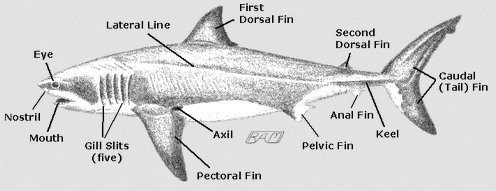
\includegraphics{Images/sharkimg.png}    
    \caption[This is another figure.] {This is another figure as an example. Please note that the Editorial Office does not allow borders around figures. Used with permission from Martin, R. Aidan.  2003. }
    \label{fig:my_label}
\end{figure}{}
\section{Placement Specifiers}

Floats are used to allow LaTeX to handle figures while maintaining the best possible presentation. However, there may be times when you disagree, and a typical example is with its positioning of figures. 
The placement specifier parameter exists as a compromise, and its purpose is to give the author a greater degree of control over where certain floats are placed. As you can see in Figure \ref{fig:my_label}A this is a shark. As you can see in \ref{tbl1} this is a something.

\begin{table}[H]
\caption{Specifier Table}
\begin{tabular}{l p{14cm} }
\hline
Specifier & Permission \\ \hline
h & Place the float here, i.e., approximately at the same point it occurs in the source text (however, not exactly at the spot) \\
\\
t & Position at the top of the page.  \\
\\
b & Position at the bottom of the page.  \\
\\
p & Put on a special page for floats only.  \\
\\
! & Override internal parameters LaTeX uses for determining "good" float positions. \\
\\
H & Places the float at precisely the location in the LaTeX code. \\
\hline
\end{tabular}
\end{table}

\newpage

%An example of a specifier parameter is shown below to force a figure into place where it is mentioned in text: 
%\begin{verbatim}
%\begin{figure}[h!]
%    \begin{center}
 %       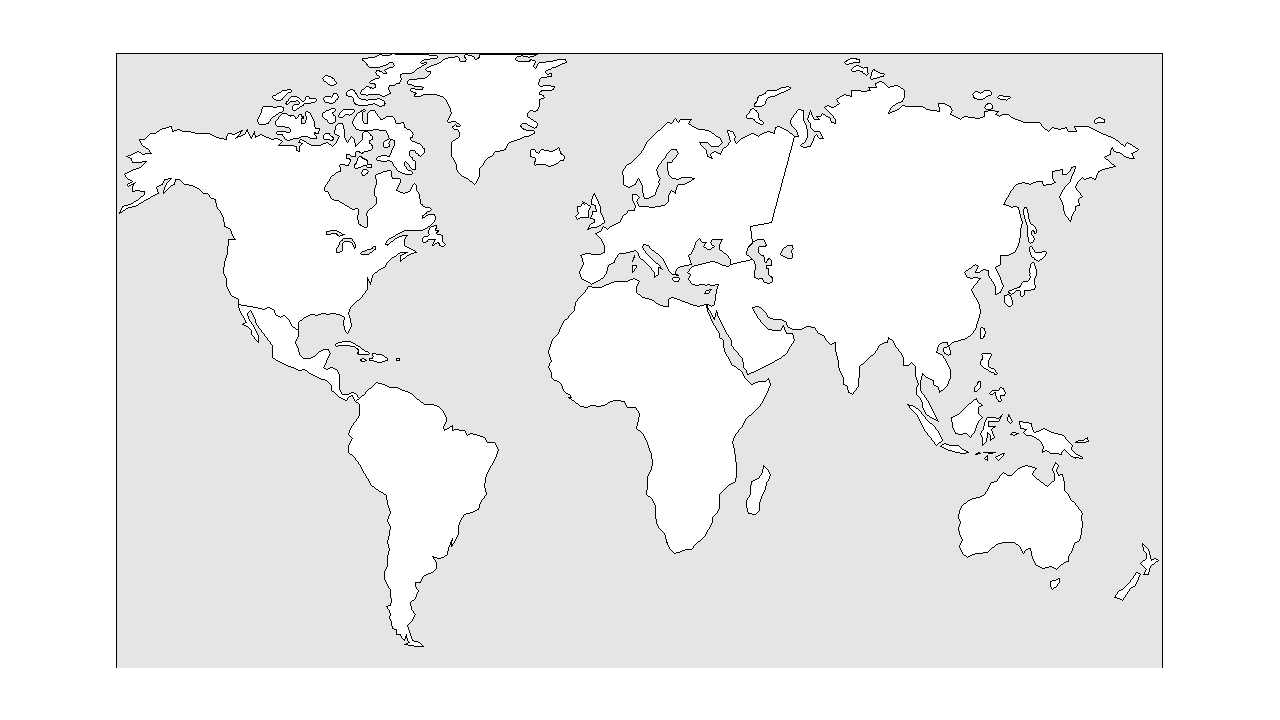
\includegraphics[width=0.9\textwidth]{./theworld.png}
%    \end{center}
%     \caption[My short caption.]{My full caption in curly brackets.}
%\end{figure}
%\end{verbatim}

% Modified from old template.

\chapter{EXAMPLES OF EDITOR/Author TOOLS}% Notice that we can use chapter/section etc breaks in the master file if we want, and then use \input instead of \include to avoid unneccessary page breaks.
If you don't see any blue or red type under this line, then you almost certainly need to include the optional ``editMode" to the document class. Thus your document class (first line) should read \verb|\documentclass[editMode]{ufdissertation}|

\authorRemark{Test! This is a remark written by the author, to themselves, for review purposes. It will be suppressed unless editMode is used in the class options.}

\editorRemark{This is an editor's remark, written by an editor in-line so that they can write into the content itself with something easy to see. But the remark will be suppressed unless editMode is used in the class options.

To get this remark to go away, simply remove ``editMode" from the documentclass options at the top of the user's tex-file. This also removes the blue Author Remarks.}
%     Stuff about using editorRemark and authorRemark commands

\chapter{SUMMARY AND CONCLUSIONS} \label{conclusion}

\section{Section Heading}

Aliquam molestie sed urna quis convallis. Aenean nibh eros, aliquam non eros in, tempus lacinia justo. In magna sapien, blandit a faucibus ac, scelerisque nec purus. Praesent fermentum felis nec massa interdum, vel dapibus mi luctus. Cras id fringilla mauris. Ut molestie eros mi, ut hendrerit nulla tempor et. Pellentesque tortor quam, mattis a scelerisque nec, euismod et odio. Mauris rhoncus metus sit amet risus mattis, eu mattis sem interdum.

\subsection{Subsection Heading}
Semper vel lorem eu, venenatis ultrices est. Nam aliquet ut erat ac scelerisque. Maecenas ut molestie mi. Phasellus ipsum magna, sollicitudin eu ipsum quis, imperdiet cursus turpis. Etiam pretium enim a fermentum accumsan. Morbi vel vehicula enim.

\subsection{Subsection Heading}
Semper vel lorem eu, venenatis ultrices est. Nam aliquet ut erat ac scelerisque. Maecenas ut molestie mi. Phasellus ipsum magna, sollicitudin eu ipsum quis, imperdiet cursus turpis. Etiam pretium enim a fermentum accumsan. Morbi vel vehicula enim.

\subsubsection{Subsubsection heading}
 Placerat cursus. Integer congue urna non massa dictum, a pellentesque arcu accumsan. Nulla posuere, elit accumsan eleifend elementum, ipsum massa tristique metus, in ornare neque nisl sed odio. Nullam eget elementum nisi. Duis a consectetur erat, sit amet malesuada sapien. Aliquam nec sapien et leo sagittis porttitor at ut lacus. Vivamus vulputate elit vitae libero condimentum dictum. Nulla facilisi. Quisque non nibh et massa ullamcorper iaculis.\cite{BigRudin}
 
 \subsubsection{Subsubsection heading}
 Placerat cursus. Integer congue urna non massa dictum, a pellentesque arcu accumsan. Nulla posuere, elit accumsan eleifend elementum, ipsum massa tristique metus, in ornare neque nisl sed odio. Nullam eget elementum nisi. Duis a consectetur erat, sit amet malesuada sapien. Aliquam nec sapien et leo sagittis porttitor at ut lacus. Vivamus vulputate elit vitae libero condimentum dictum. Nulla facilisi. Quisque non nibh et massa ullamcorper iaculis.\cite{BigRudin}
 
 \section{Section Heading}
Aliquam molestie sed urna quis convallis. Aenean nibh eros, aliquam non eros in, tempus lacinia justo. In magna sapien, blandit a faucibus ac, scelerisque nec purus. Praesent fermentum felis nec massa interdum, vel dapibus mi luctus. Cras id fringilla mauris. Ut molestie eros mi, ut hendrerit nulla tempor et. Pellentesque tortor quam, mattis a scelerisque nec, euismod et odio. Mauris rhoncus metus sit amet risus mattis, eu mattis sem interdum.
% Modified from old template.



\end{document}

